%                                                                 aa.dem
% AA vers. 9.1, LaTeX class for Astronomy & Astrophysics
% demonstration file
%                                                       (c) EDP Sciences
%-----------------------------------------------------------------------
%
%\documentclass[referee]{aa} % for a referee version
%\documentclass[onecolumn]{aa} % for a paper on 1 column  
%\documentclass[longauth]{aa} % for the long lists of affiliations 
%\documentclass[letter]{aa} % for the letters 
%\documentclass[bibyear]{aa} % if the references are not structured 
%                              according to the author-year natbib style

%
\documentclass{aa}  

%
\usepackage{graphicx}
%%%%%%%%%%%%%%%%%%%%%%%%%%%%%%%%%%%%%%%%
\usepackage{txfonts}
\usepackage{hyperref}
%%%%%%%%%%%%%%%%%%%%%%%%%%%%%%%%%%%%%%%%
%\usepackage[options]{hyperref}
% To add links in your PDF file, use the package "hyperref"
% with options according to your LaTeX or PDFLaTeX drivers.
%

\begin{document} 

\title{Magnetized Polish doughnuts revisited}

%   \subtitle{}

   \author{Sergio Gimeno\inst{1}   \and Jos\'e A.~Font\inst{1,2} }

   \institute{Departamento de Astronom\'{\i}a y Astrof\'{\i}sica, Universitat de Val\`encia, Dr. Moliner 50, 46100, Burjassot (Val\`encia), Spain.\\
              \email{sergiso@alumni.uv.es}
         \and
             Observatori Astron\`omic, Universitat de Val\`encia, C/ Catedr\'atico Jos\'e Beltr\'an 2, 46980, Paterna (Val\`encia), Spain. \\
             \email{j.antonio.font@uv.es}
             }

   \date{}

% \abstract{}{}{}{}{} 
% 5 {} token are mandatory
 
  \abstract
  % context heading (optional)
  % {} leave it empty if necessary  
   {}
  % aims heading (mandatory)
   {bla}
  % methods heading (mandatory)
   {bla}
  % results heading (mandatory)
   {bla}
  % conclusions heading (optional), leave it empty if necessary 
   {}

   \keywords{keywords here}

   \maketitle

%%%%%%%%%%%
\section{Introduction}
%%%%%%%%%%%

% From Qian et al: 
% We construct a new family of analytic models of black hole accretion disks in dynamical equilibria. 
% Our construction is based on assuming distributions of angular momentum and entropy. For a 
% particular choice of the distribution of angular momentum, we calculate the shapes of equipressure 
% surfaces. The equipressure surfaces we find are similar to those in thick, slim and thin disks, and
% to those in ADAFs.
% Models of tori described here may be useful not only for accretion
% disks but also for tori that formin the latest stages of neutron
% star binary mergers. This is relevant for gamma ray bursts (Witt
% et al. 1994) and gravitational waves (Baiotti et al. 2008).

% From Komissarov:
% The dynamics of accretion discs around galactic and extragalactic black holes may be influenced
% by their magnetic field. In this paper, we generalize the fully relativistic theory of
% stationary axisymmetric tori in Kerr metric of Abramowicz, Jaroszynski&Sikora by including
% strong toroidal magnetic field and construct analytic solutions for barotropic tori with constant
% angular momentum. This development is particularly important for the general relativistic
% computational magnetohydrodynamics that suffers from the lack of exact analytic solutions
% that are needed to test computer codes.



Matter accretion on to a black hole is the most efficient form of energy production known in nature. The conversion of the
gravitational energy of the infalling matter into heat and radiation may reach efficiencies
of about 43\% in the case of rotating (Kerr) black holes. For this reason, systems formed 
by a black hole surrounded by an accretion disk are deemed responsible for many of the most energetic astronomical phenomena observed in the cosmos.
In particular, (geometrically) thick accretion disks are believed to be present in quasars and other active galactic nuclei, some 
X-ray binaries and microquasars, as well as in the central engine of gamma-ray bursts.

The investigation of such systems, either by analytical or numerical means, may rely on the ability to construct suitable 
representations based on physical assumptions. The construction of equilibrium models of stationary disks around black holes has a long tradition (see~\cite{Abramowicz:2013} and references therein). In particular, the so-called ``Polish doughnuts"~\citep{Abramowicz:1978,Kozlowski:1978} provide a  very general method to build equilibrium configurations of perfect fluid matter  
 orbiting around a Kerr black hole. This fully relativistic model assumes that the disk is non-magnetized and that the matter obeys a  constant specific angular momentum distribution. This method was extended by~\cite{Komissarov:2006}  by adding a purely azimuthal magnetic 
 field to build magnetized tori around rotating black holes. Assuming different distributions of angular momentum in the disks, \citet{Qian:2009} presented a method to build sequences of black hole thick accretion disks in dynamical equilibria, restricted to the purely hydrodynamical case. Building on this work, we discuss here the extension of the
models of~\citet{Qian:2009} to disks endowed with a purely toroidal magnetic field. For the particular case of constant angular momentum distributions our method shows good agreement with the results of~\citet{Komissarov:2006}.

The organization of the paper is as follows:
We assume that the test-fluid approximation holds, neglecting the self-gravity of the fluid, and assume that the space-time is described by the Kerr metric. We use geometrized units where $G = c = 1$.

%%%%%%%%%%%
\section{Framework}
%%%%%%%%%%%

Equilibrium tori around Kerr black holes are built assuming that the spacetime gravitational potentials and the fluid fields are stationary and axisymmetric. In all the derivations presented below, the Kerr metric is implicitely written using standard Boyer-Lindquist coordinates. It is convenient to introduce a number of relevant characteristic radii, such as the radius
of the marginally stable circular orbit, $r_{\rm ms}$, and the radius of the marginally bound circular orbit, $r_{\rm mb}$, given by
\begin{eqnarray}
r_{\rm ms} &=& M\,\left(3+Z_2-\left[(3-Z_1)(3+Z_1+2Z_2)\right]^{1/2})\right)\,,
\\
r_{\rm mb} &=& 2M\,\left(  1-\frac{a_*}{2} + \sqrt{1-a_*} \right)\,,
\end{eqnarray}
where $Z_1=1+(1-a_*^2)^{1/3}[(1+a_*)^{1/3}+(1-a_*)^{1/3}]$, $Z_2=(3a_*^2+Z_1^2)^{1/2}$, and $a_*=a/M$, with $a$ and $M$ being the spin Kerr parameter and the black hole mass.

%%%%%%%%%%%%%%%%%%%%%%%%
\subsection{Distribution of angular momentum}
%%%%%%%%%%%%%%%%%%%%%%%%

We introduce the specific angular momentum $l$ and the angular velocity $\Omega$ employing the standard definitions,
\begin{equation}
l = - \frac{u_{\phi}}{u_t}, \;\;\; \Omega = \frac{u^{\phi}}{u^t},
\end{equation}
where $u^{\mu}$ is the fluid four-velocity.
%
%\footnote{In Kerr-Schild coordinates. Although the use of the Boyer-Lindquist coordinates yields exactly the same mathematical derivation and results.}.
%
The relationship between $l$ and $\Omega$ is given by the equations
\begin{equation}
l = - \frac{\Omega g_{\phi\phi} + g_{t\phi}}{\Omega g_{t\phi} + g_{tt}}, \;\;\; \Omega = - \frac{l g_{tt} + g_{t\phi}}{l g_{t\phi} + g_{\phi\phi}},
\end{equation}
where $g_{\mu\nu}$ is the metric tensor and we are assuming circular motion, i.e. the four-velocity can be written as
\begin{equation}
u^{\mu} = (u^t, 0, 0, u^{\phi})\,.
\end{equation}
We also introduce the Keplerian angular momentum (for prograde motion) in the equatorial plane $l_{\mathrm{K}}$. 
\begin{equation}\label{eq:kepler}
l_{\mathrm{K}}(r) = \frac{M^{1/2}(r^{2}-2aM^{1/2}r^{1/2}+a^{2})}{r^{3/2}-2Mr^{1/2}+aM^{1/2}}\,.
\end{equation}

\cite{Jaroszynski:1980} argued that the slope of the specific angular momentum should range between two cases, $l = \mathrm{const.}$ and $\Omega = \mathrm{const}$. Following \citet{Qian:2009} we assume an angular momentum distribution ansatz given by  
\begin{equation}
l (r,\theta) = \left\{ \label{eq:ansatz} 
  \begin{array}{lr}
    l_0 \left(\frac{l_{\mathrm{K}}(r)}{l_0}\right)^{\beta}\sin^{2\gamma}{\theta} &  \text{for } r \geq r_{\mathrm{ms}}\\
    l_{\mathrm{ms}}(r)\sin^{2\gamma}{\theta} & \text{for } r < r_{\mathrm{ms}}
  \end{array}
\right.
\end{equation}
where constants $l_0$ and $l_{\mathrm{ms}}(r)$ are defined by $l_0 \equiv \eta l_{\mathrm{K}}(r_{\mathrm{ms}})$ and $l_{\mathrm{ms}}(r) \equiv l_0 [l_{\mathrm{K}}(r_{\mathrm{ms}})/l_0]^{\beta}$. Therefore, the model for the distribution of angular momentum has three parameters $(\beta, \gamma, \eta)$, whose range of variation is given by~\citep{Qian:2009}
\begin{equation}
0 \leq \beta \leq 1, \quad -1 \leq \gamma \leq 1, \quad 1 \leq \eta \leq \eta_{\mathrm{max}},
\end{equation}
with $\eta_{\mathrm{max}} = l_{\mathrm{K}}(r_{\mathrm{mb}})/l_{\mathrm{K}}(r_{\mathrm{ms}})$. In this paper we choose $\eta = \eta_{\mathrm{max}}$, then we can write $l_0$ as $l_0 = l_{\mathrm{K}}(r_{\mathrm{mb}})$. We take this choice because [explicar que esta eleccion hace que el momento angular esté comprendido entre lmb y lms para variaciones de beta entre 0 y 1. Además los discos de momento angular constante que empiezan en el cusp, no tienen borde externo para l = lmb]

%%%%%%%%%%%%%%%%
\subsection{Magnetized disks}
%%%%%%%%%%%%%%%%

The equations of ideal general relativistic MHD are $\nabla_{\mu} T^{\mu\nu} = 0$, $\nabla_{\mu} \,^\ast F^{\mu\nu} = 0$, and 
$\nabla_{\mu} (\rho u^{\mu}) = 0$, 
%\begin{equation}\label{eq:e-m_cons}
%\nabla_{\mu} T^{\mu\nu} = 0,
%\end{equation}
%\begin{equation}\label{eq:cons_faraday}
%\nabla_{\mu} \ast F^{\mu\nu} = 0,
%\end{equation}
%\begin{equation}\label{eq:continuity}
%\nabla_{\mu} (\rho u^{\mu}) = 0,
%\end{equation}
where $\nabla_{\mu}$ is the covariant derivative and
\begin{equation}\label{eq:e-m_tensor}
T^{\mu\nu} = (w + b^2)u^{\mu}u^{\nu} + \left(p + \frac{1}{2}b^2\right)g^{\mu\nu} - b^{\mu}b^{\nu},
\end{equation}
is the energy-momentum tensor of a magnetized perfect fluid, $w$ and $p$ being the fluid enthalpy and pressure, respectively. 
Moreover,
%\begin{equation}
$^\ast F^{\mu\nu} = b^{\mu}u^{\nu} - b^{\nu}u^{\mu}$
%\end{equation}
is the (dual of the) Faraday tensor relative to an observer with four-velocity $u^{\mu}$, and $b^{\mu}$ is the magnetic field in that frame, with
$b^2=b^{\mu}b_{\mu}$. Assuming the magnetic field is purely azimuthal, i.e.~$b^r = b^{\theta} = 0$,
and taking into account that the flow is stationary and axisymmetric, the conservation of the current density and of the Faraday tensor follow. Contracting Eq.~\eqref{eq:e-m_tensor} with the projection tensor $h^{\alpha}_{\beta} = \delta^{\alpha}_{\beta} + u^{\alpha}u_{\beta}$, we arrive at
\begin{equation}
(w + b^2)u_{\nu}\partial_i u^{\nu} + \partial_i\left(p + \frac{b^2}{2}\right) - b_{\nu}\partial_i b^{\nu}=0\,,
\end{equation}
where $i = r, \theta$. Following~\cite{Komissarov:2006} we rewrite this equation in terms of the specific angular momentum $l$ and the angular velocity $\Omega$, to obtain
\begin{equation}\label{eq:diff_ver}
\partial_i(\ln u_t|) - \frac{\Omega \partial_i l}{1-l\Omega} + \frac{\partial_i p}{w} + \frac{\partial_i(\mathcal{L}b^2)}{2\mathcal{L}w} = 0\,,
\end{equation}
where $\mathcal{L} = g_{t\phi}^2 - g_{tt}g_{\phi\phi}$.
To integrate Eq.~\eqref{eq:diff_ver} we first assume a barotropic equation of state $w = w(p)$ of the form
\begin{equation}\label{eq:eos_fluid}
p = K w^{\kappa},
\end{equation}
with $K$ and $\kappa$ constants.
Then, we define the magnetic pressure as $p_{\mathrm{m}} = b^2/2$, and introduce the definitions $\tilde{p}_{\mathrm{m}} = \mathcal{L} p_{\mathrm{m}}$ and $\tilde{w} = \mathcal{L} w$, in order to write an analog equation to Eq.~\eqref{eq:eos_fluid} for $\tilde{p}_{\mathrm{m}}$~\citep{Komissarov:2006}
\begin{equation}\label{eq:eos_mag_tilde}
\tilde{p}_{\mathrm{m}} = K_{\mathrm{m}} \tilde{w}_{\mathrm{m}}^{\eta},
\end{equation}
or, in terms of the magnetic pressure $p_{\mathrm{m}}$
\begin{equation}\label{eq:eos_mag}
p_{\mathrm{m}} = K_{\mathrm{m}} \mathcal{L}^{\eta-1} w^{\eta},
\end{equation}
where $K_{\mathrm{m}}$ and $\eta$ are constants.
This particular choice of relationships, $w = w(p)$ and $\tilde{w} = \tilde{w}(\tilde{p}_{\mathrm{m}})$, fulfill the general relativistic version of the von Zeipel theorem for a toroidal magnetic field~\citep{vonZeipel:1924, Zanotti:2015}, i.e.~the surfaces of constant $\Omega$ and constant $l$ coincide.

Integrating Eq.~\eqref{eq:diff_ver} we obtain
\begin{equation}\label{eq:pre_full_int}
\ln |u_t| - \int^l_0 \frac{\Omega \mathrm{d}l}{1 - \Omega l} + \int^p_0 \frac{\mathrm{d}p}{w} + \int_0^{\tilde{p}_{\mathrm{m}}} \frac{\mathrm{d}\tilde{p}_{\mathrm{m}}}{\tilde{w}} = \mathrm{const}.
\end{equation}
On the surface of the disk, and particularly on its inner edge, the conditions
$p = \tilde{p}_{\mathrm{m}} = 0, \; u_t = u_{t, \mathrm{in}}, \; l = l_{\mathrm{in}}$
are satisfied and, therefore, the integration constant is simply given by
\begin{equation}
\mathrm{const.} = \ln |u_t| - \int^l_{l_\mathrm{in}} \frac{\Omega \mathrm{d}l}{1 - \Omega l}\,.
\end{equation}
We can also introduce the total (gravitational plus centrifugal) potential $W$~\citep{Abramowicz:1978} and write the integral form of the equation of motion as
\begin{equation}\label{eq:potential}
W - W_{\mathrm{in}} = \ln|u_t| - \ln|u_{t,\mathrm{in}}| - \int^{l}_{l_{\mathrm{in}}} \frac{\Omega \mathrm{d}l}{1 - \Omega l},
\end{equation}
where $W_{\mathrm{in}}$ is the potential at the inner edge of the disk (in the equatorial plane). With this definition, we can write Eq.~\eqref{eq:pre_full_int} as
\begin{equation}\label{eq:full_int}
W - W_{\mathrm{in}} = \int^p_0 \frac{\mathrm{d}p}{w} + \int_0^{\tilde{p}_{\mathrm{m}}} \frac{\mathrm{d}\tilde{p}_{\mathrm{m}}}{\tilde{w}},
\end{equation}
which for a barotropic equation of state can be easily integrated to give
\begin{equation}\label{eq:pre_enthalpy_eq}
W - W_{\rm{in}} + \frac{\kappa}{\kappa - 1}\frac{p}{w} + \frac{\eta}{\eta - 1}\frac{p_{\mathrm{m}}}{w} = 0\,.
\end{equation}
Replacing $p$ and $p_{\mathrm{m}}$ by equations \eqref{eq:eos_fluid} and \eqref{eq:eos_mag}, the previous equation reduces to
\begin{equation}\label{eq:enthalpy_eq}
W - W_{\rm{in}} + \frac{\kappa}{\kappa - 1} K w^{\kappa - 1} + \frac{\eta}{\eta - 1}K_{\mathrm{m}}(\mathcal{L} w)^{\eta - 1} = 0,
\end{equation}
which relates the distribution of potential with the distribution of enthalpy.

%Finally, we assume a polytropic equation of state given by
%\begin{equation}\label{eq:density_eq}
%p = K \rho^{\kappa}
%\end{equation}
%where $\rho$ is the fluid density.

%%%%%%%%%%%%
\section{Methodology}
%%%%%%%%%%%%

\subsection{Building the disk}

To construct the disks we follow the approach described in \citet{Qian:2009}. First, we find the radial location of the cusp and the center of the disk in the equatorial plane, $r_{\mathrm{cusp}}$ and $r_{\mathrm{c}}$, defined as the solutions to the equation $l(r) - l_{\mathrm{K}} = 0$.
Next, we compute the partial derivatives of the potential, Eq.~\eqref{eq:potential}
\begin{equation}\label{eq:radial_der_pot}
\partial_r W = \partial_r \ln|u_t| - \frac{\Omega \partial_rl}{1 - \Omega l}\,,
\end{equation}
and
\begin{equation}\label{eq:polar_der_pot}
\partial_{\theta} W = \partial_{\theta} \ln|u_t| - \frac{\Omega \partial_{\theta}l}{1 - \Omega l}\,.
\end{equation}
Then, we integrate the radial partial derivative of the potential along the segment $[r_{\mathrm{cusp}}, r_{\mathrm{c}}]$ (assuming $W_{\mathrm{cusp}} = 0$) at the equatorial plane, thus obtaining the equatorial distribution of the potential between $r_{\mathrm{cusp}}$ and $r_{\mathrm{c}}$
\begin{equation}\label{eq:equatorial_pot}
W_{\mathrm{eq}}(r) = \int^{r}_{r_{\mathrm{cusp}}}\left(\partial_r \ln|u_t| - \frac{\Omega \partial_rl}{1 - \Omega l}\right).
\end{equation}
Following \citet{Qian:2009} we can divide equations \eqref{eq:radial_der_pot} and \eqref{eq:polar_der_pot} to obtain
\begin{equation}\label{eq:F}
F(r, \theta) = -\frac{\partial_r W}{\partial_{\theta} W} = \frac{\mathrm{d}\theta}{\mathrm{d}r}\,,
\end{equation}
which is an ordinary differential equation that can be integrated to obtain the location of the equipotential surfaces.

Next, we choose all the initial values for the integration of the equation \eqref{eq:F} to be between $r_{\mathrm{cusp}}$ and $r_{\mathrm{c}}$ ($\theta = \pi / 2$). Since we are only interested in the surfaces inside the Roche lobe, our choice of initial values provides us a mapping of the equipotential surfaces of the torus. Given that we have already obtained both the equipotential surfaces which cross the segment $[r_{\mathrm{cusp}}, r_{\mathrm{c}}]$ and the potential distribution there, we found the potential distribution for the torus.
Once we have the potential distribution, we can find the gas pressure at the center, from equation \eqref{eq:enthalpy_eq}
\begin{equation}
p_{\mathrm{c}} = w_{\mathrm{c}}(W_{\mathrm{in}} - W_{\mathrm{c}})\left(\frac{\kappa}{\kappa - 1} + \frac{\eta}{\eta - 1}\frac{1}{\beta_{\mathrm{c}}}\right)^{-1},
\end{equation}
where $w_{\mathrm{m}}$ is the enthalpy at the disk center and
\begin{equation}\label{eq:beta_eq}
\beta = p/p_{\mathrm{m}},
\end{equation}
is the magnetization parameter (being $\beta_{\mathrm{m}}$ the magnetization parameter at the disk center). By this definition, we can find the magnetic pressure at the disk center,
\begin{equation}
p_{\mathrm{m_{\mathrm{c}}}} = p_{\mathrm{c}}/\beta_{\mathrm{c}}
\end{equation}
With the pressures at the center, we can also find the constants $K$ and $K_{\mathrm{m}}$ using the equations \eqref{eq:eos_fluid} and \eqref{eq:eos_mag}. And, for a given inner radius of the disk $r_{\mathrm{in}}$ we can find the potential $W_{\mathrm{in}}$. We now have all the elements required to find the enthalpy distribution (equation \eqref{eq:enthalpy_eq}), the pressure and magnetic pressure distribution (equations \eqref{eq:eos_fluid} and \eqref{eq:eos_mag}), and the density (equation \eqref{eq:density_eq}).

\subsection{Numerical code}

For the integration of equation \eqref{eq:equatorial_pot} we use the composite Simpson's rule, it is important to use a very small step of integration, because the slope is very steep. In this work, we use a step $h = 10^{-6}$ . A bigger step gives an unacceptable lack of accuracy, we tested that fact by comparison with the analytic, constant angular momentum case.

To integrate the ordinary differential equation \eqref{eq:F} we use the RK4 method. Here is also important to choose a suitable step of integration, specially at the outer end of the disk, this is because the equation \eqref{eq:F} diverges of the equatorial plane (the equipotential surfaces crosses the equatorial plane perpendicularly).

\subsection{Parameter space}

As in \citet{Komissarov:2006}, in this paper we have chosen the exponents $\kappa = \eta = 4/3$ and the enthalpy at the disk center $w_{\mathrm{c}} = 0$. That leaves us the magnetization parameter $\beta$, the parameters of the angular momentum distribution $\beta$ and $\gamma$, the BH spin parameter $a$ and the inner radius of the disk $r_{\mathrm{in}}$. This allows us to control the size, shape, thickness and magnetization of the disk.

%%%%%%%%%
\section{Results}
%%%%%%%%%

Figure~\ref{komissarov} corresponds to the same constant specific angular momentum model presented by~\citet{Komissarov:2006}. The comparison shows that our approach can reproduce those previous results with good agreement. {\bf Complete description.}

\begin{figure*}
\centering
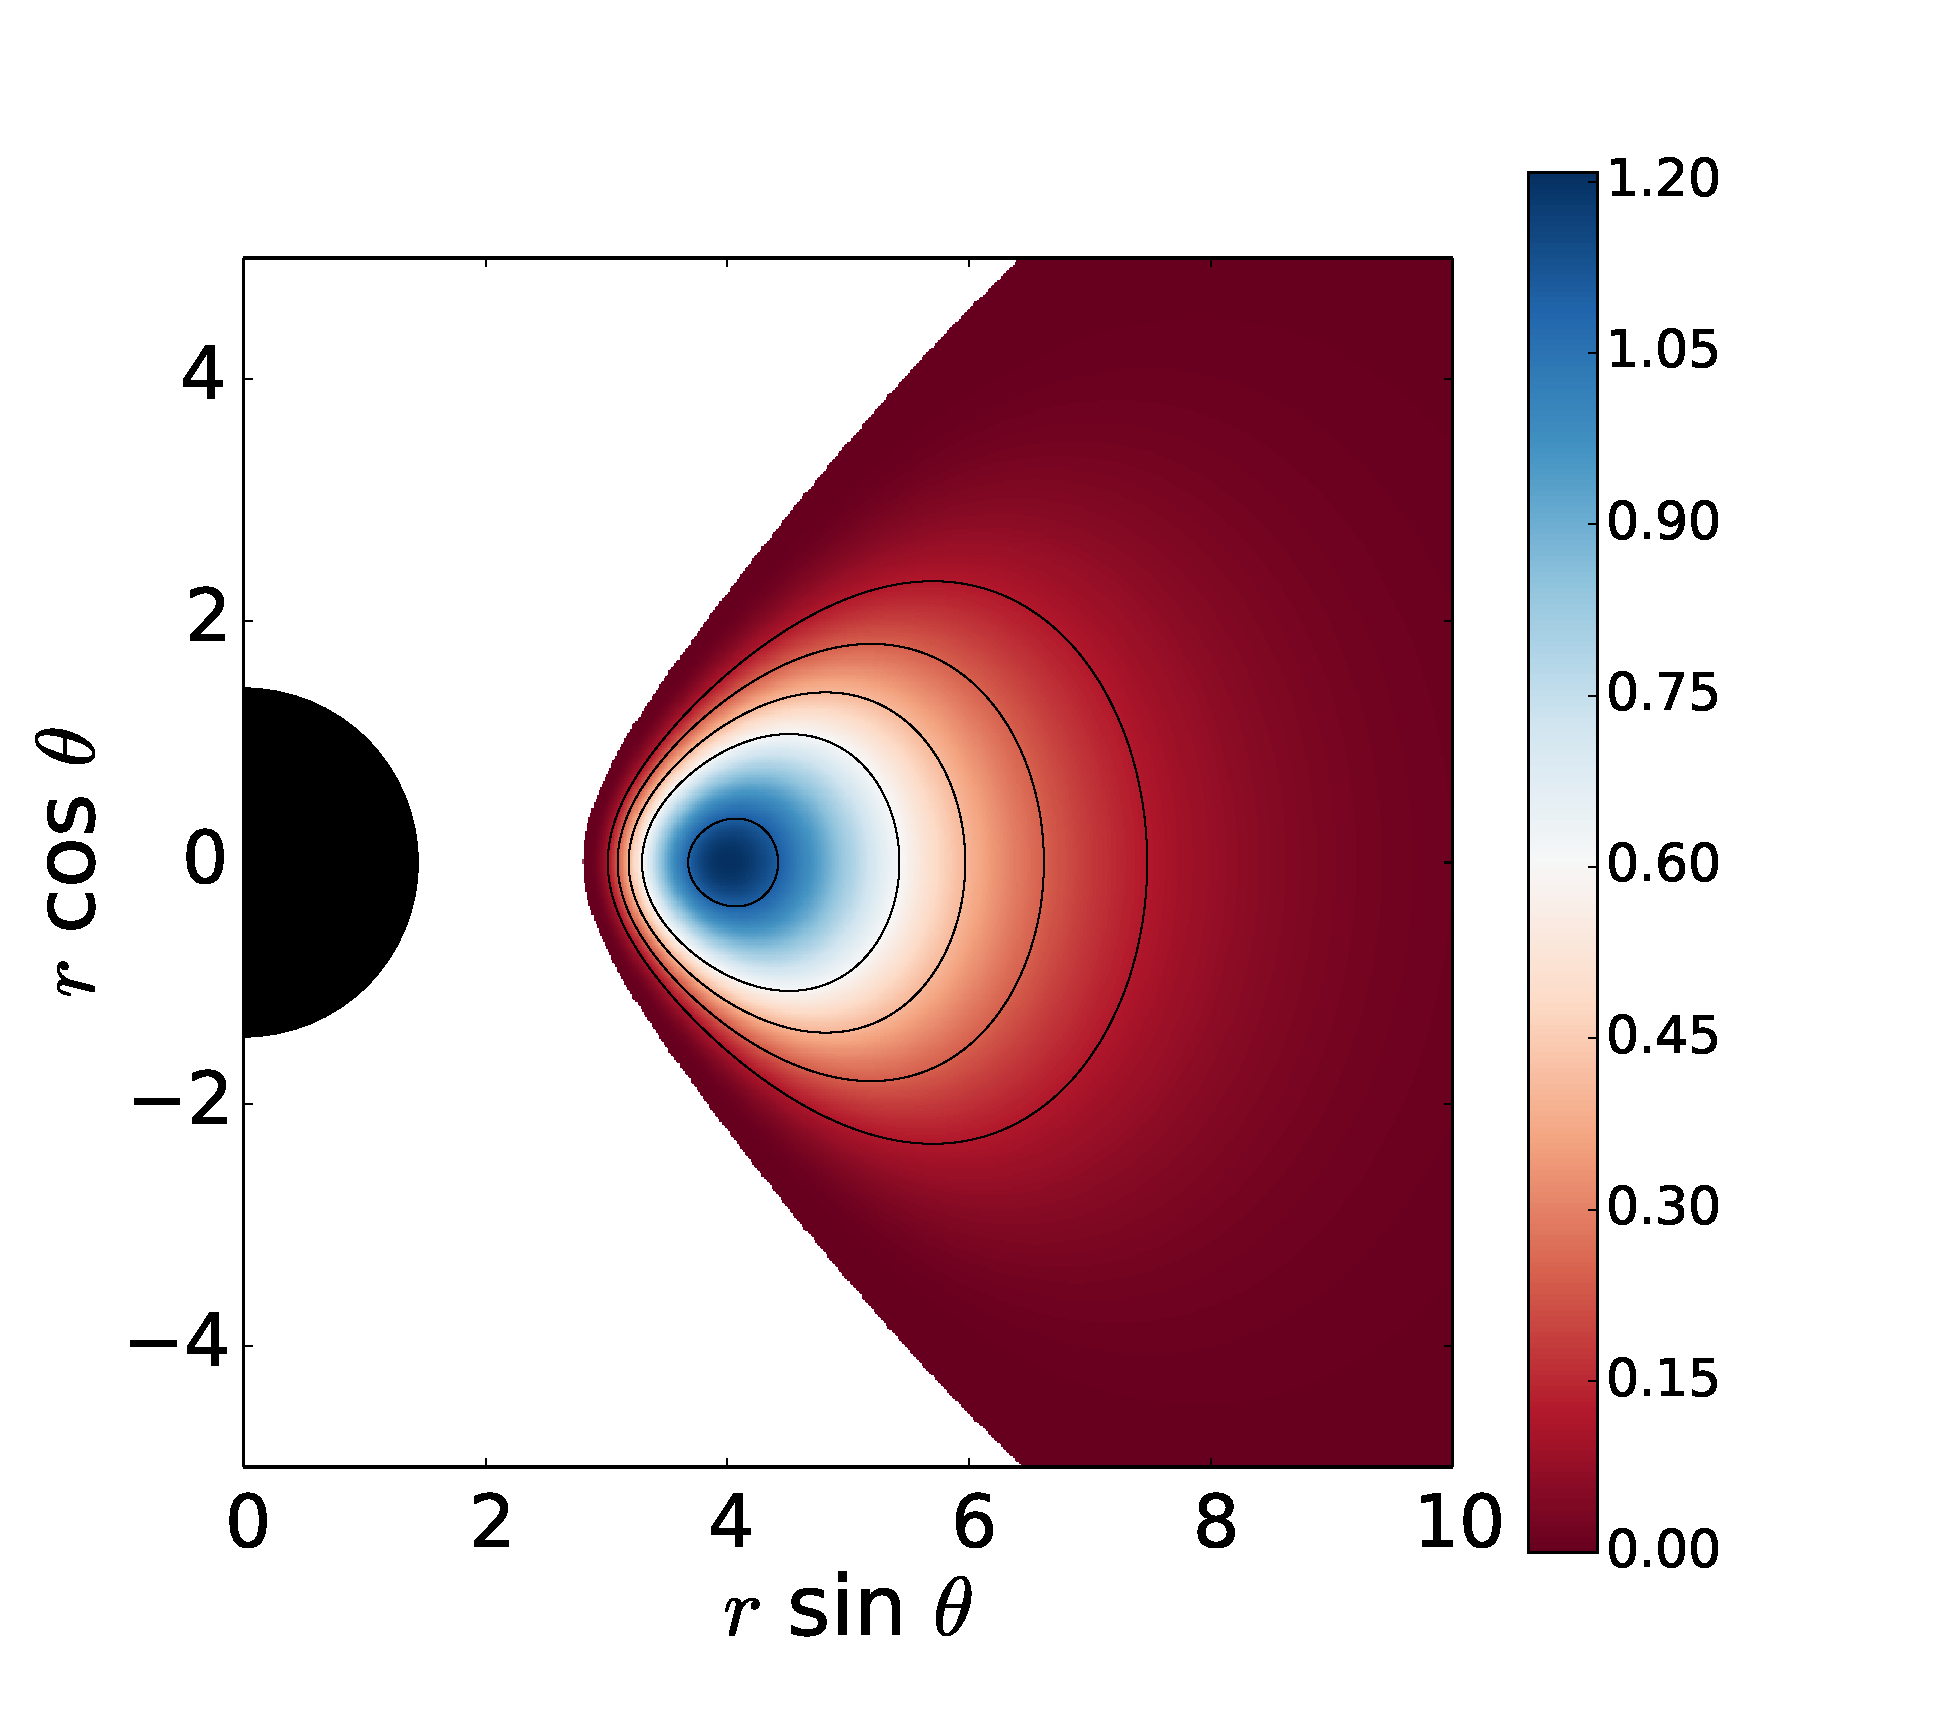
\includegraphics[scale=0.32]{images/1_A.pdf}
\hspace{-1.2cm}
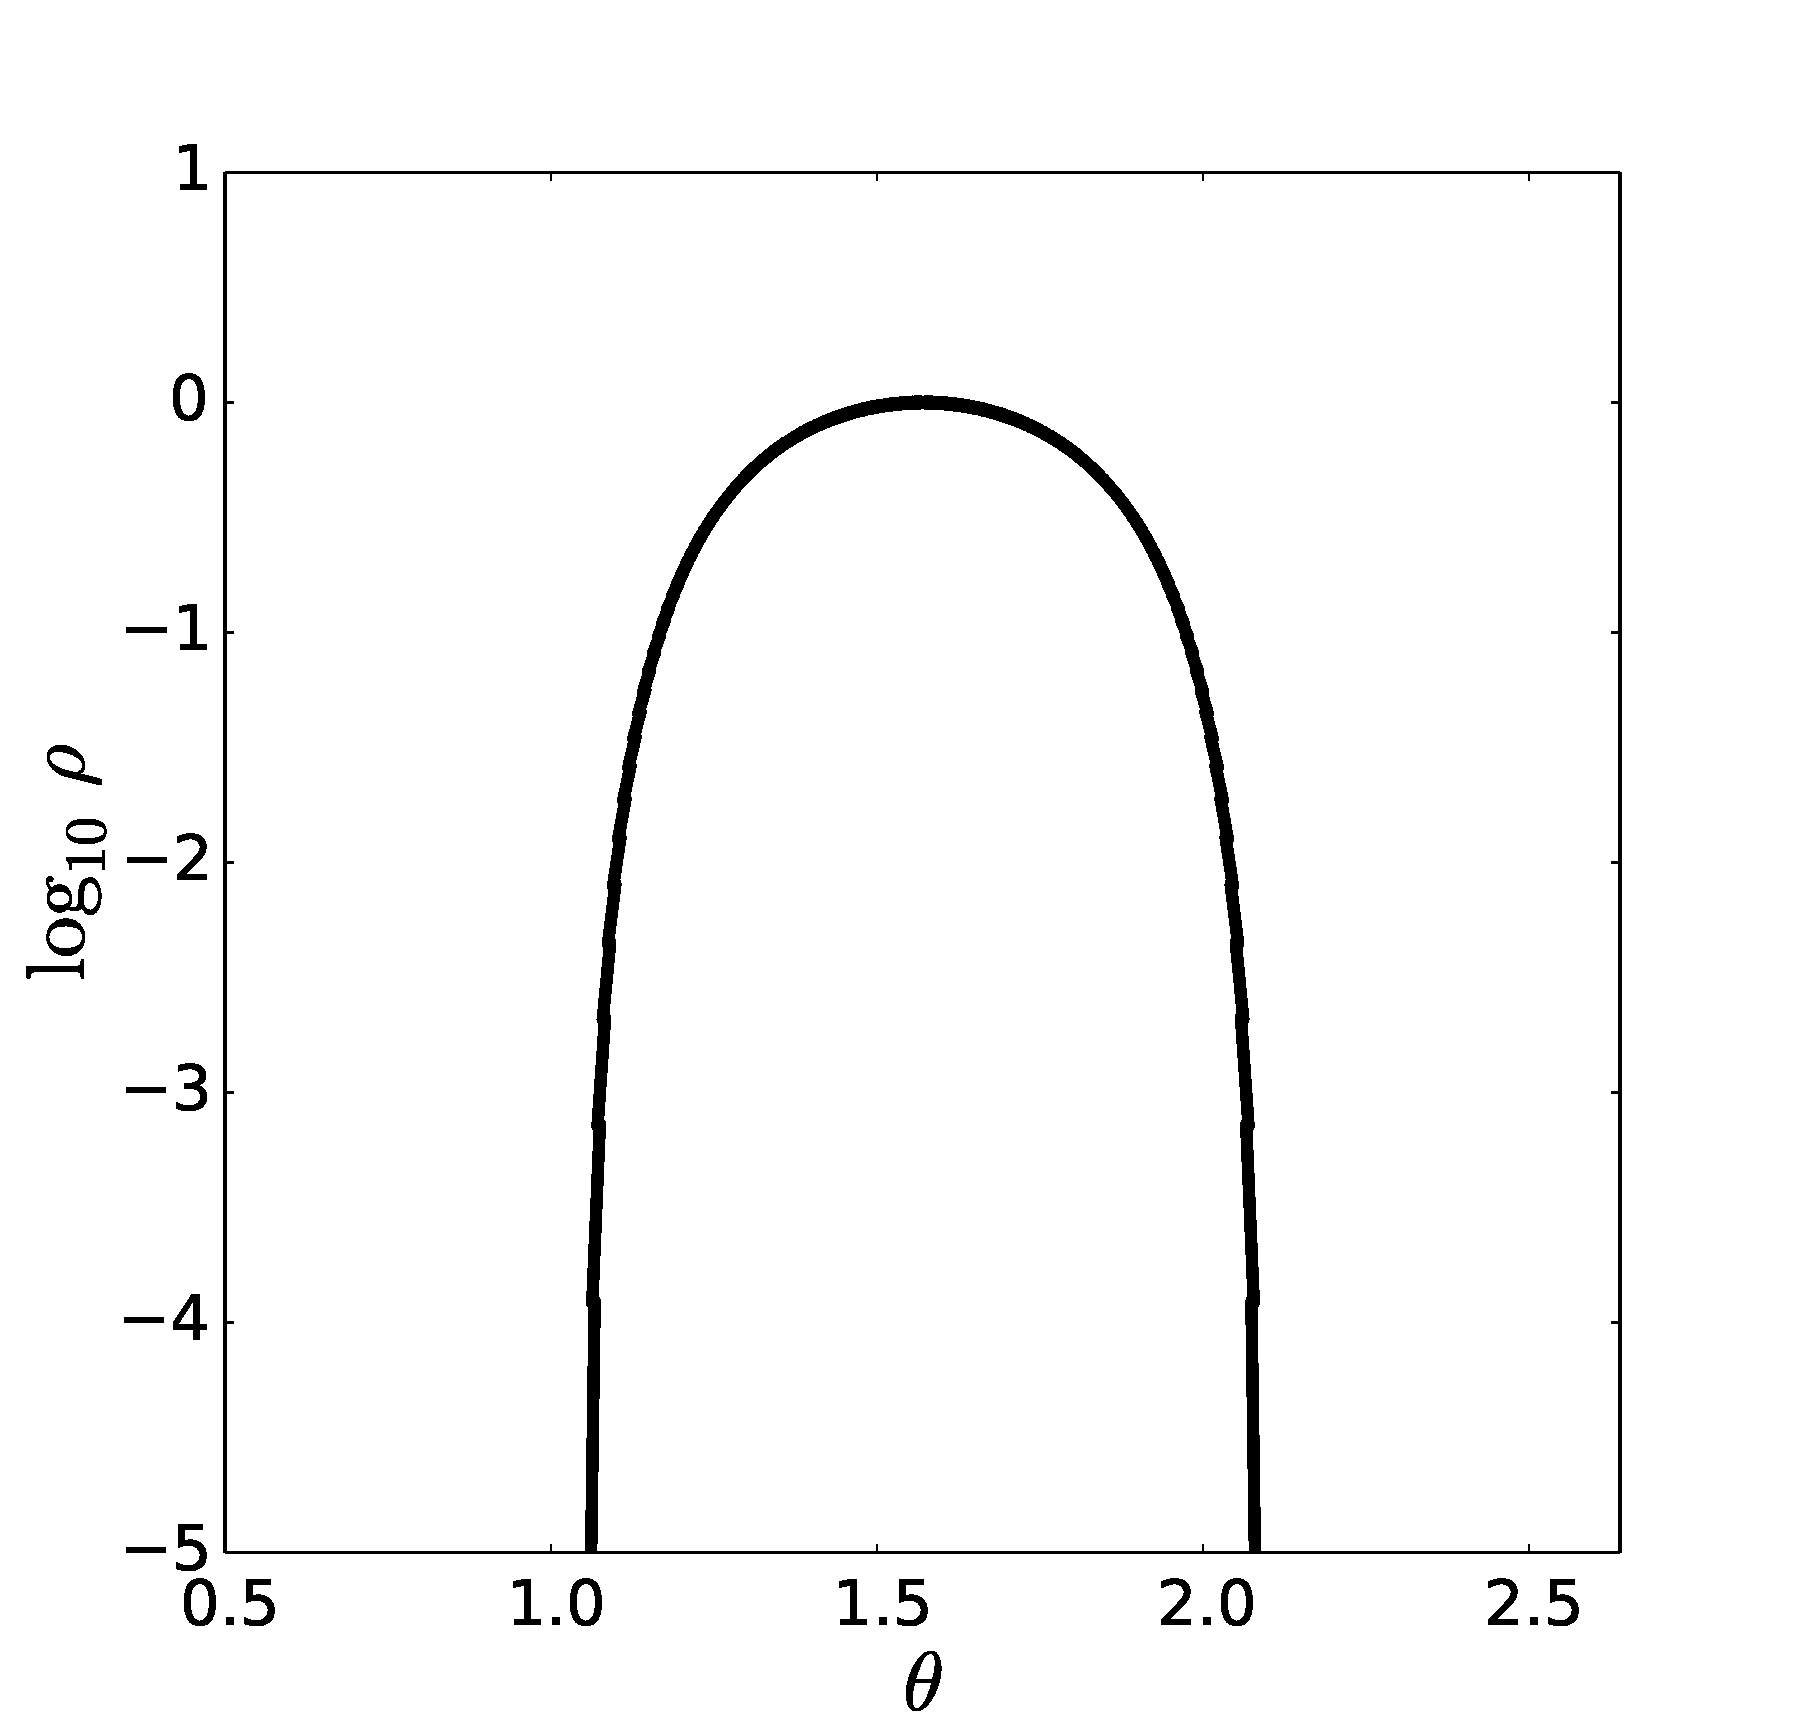
\includegraphics[scale=0.32]{images/1_B.pdf}
\hspace{-0.8cm}
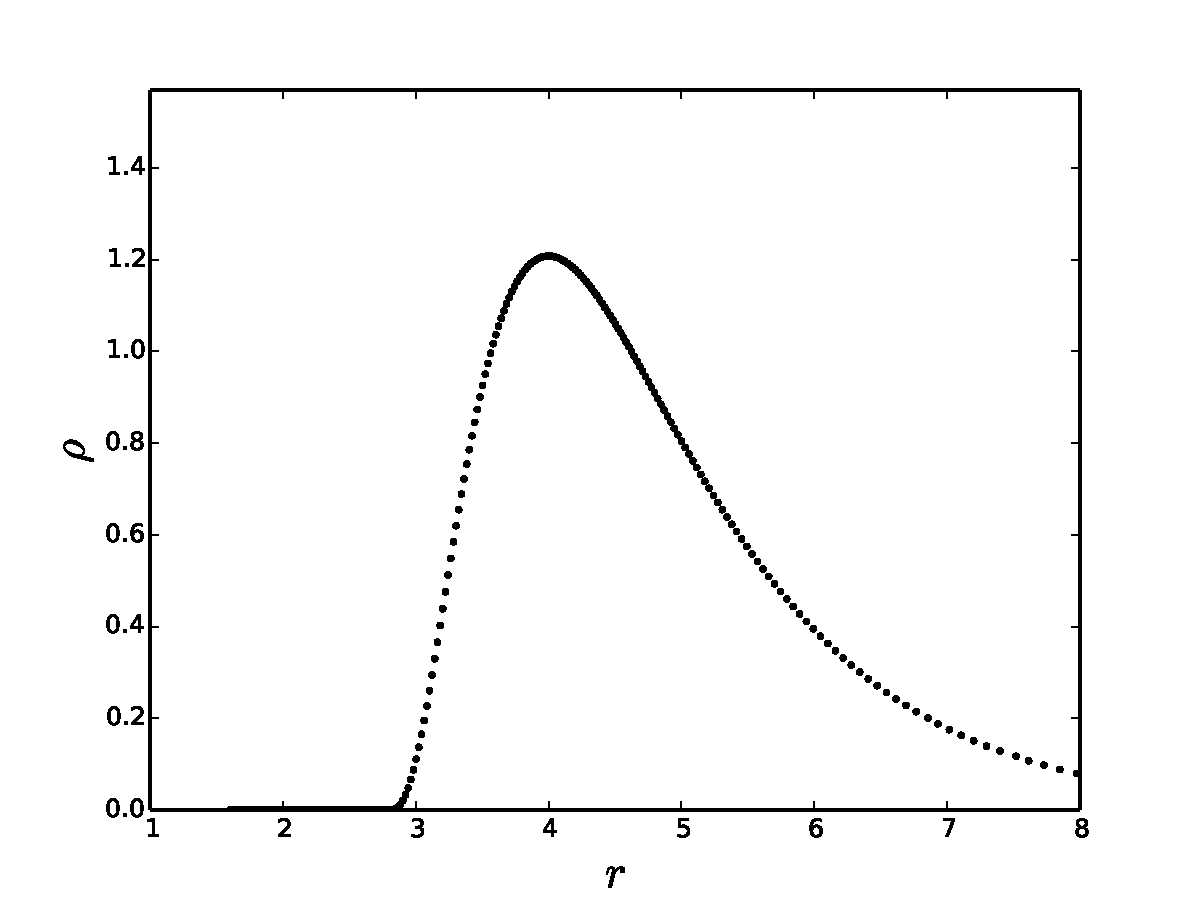
\includegraphics[scale=0.32]{images/1_C.pdf}
\caption{Comparison with Komissarov's solution for a constant angular momentum model.}
           \label{komissarov}%
 \end{figure*}


%\begin{figure*}
%\centering
%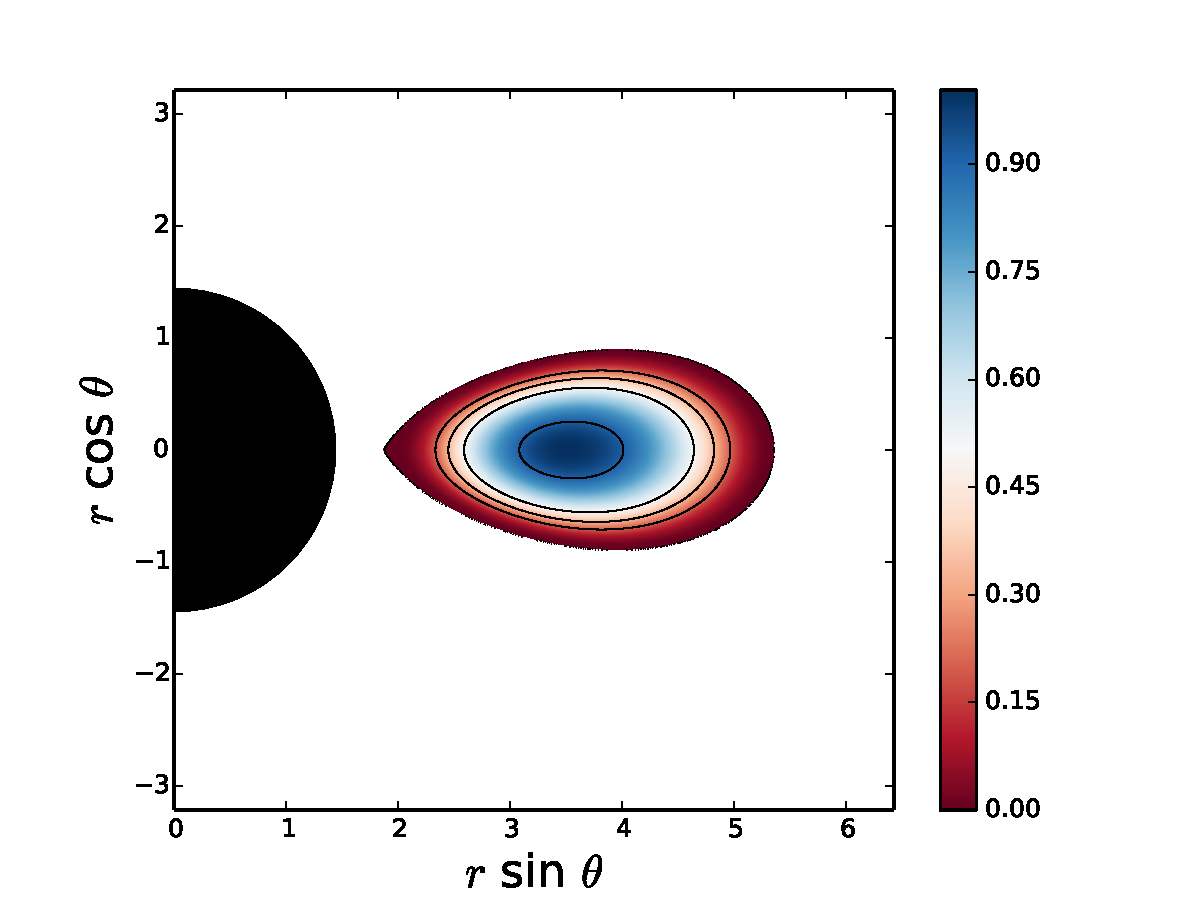
\includegraphics[scale=0.4]{images/1.pdf}
%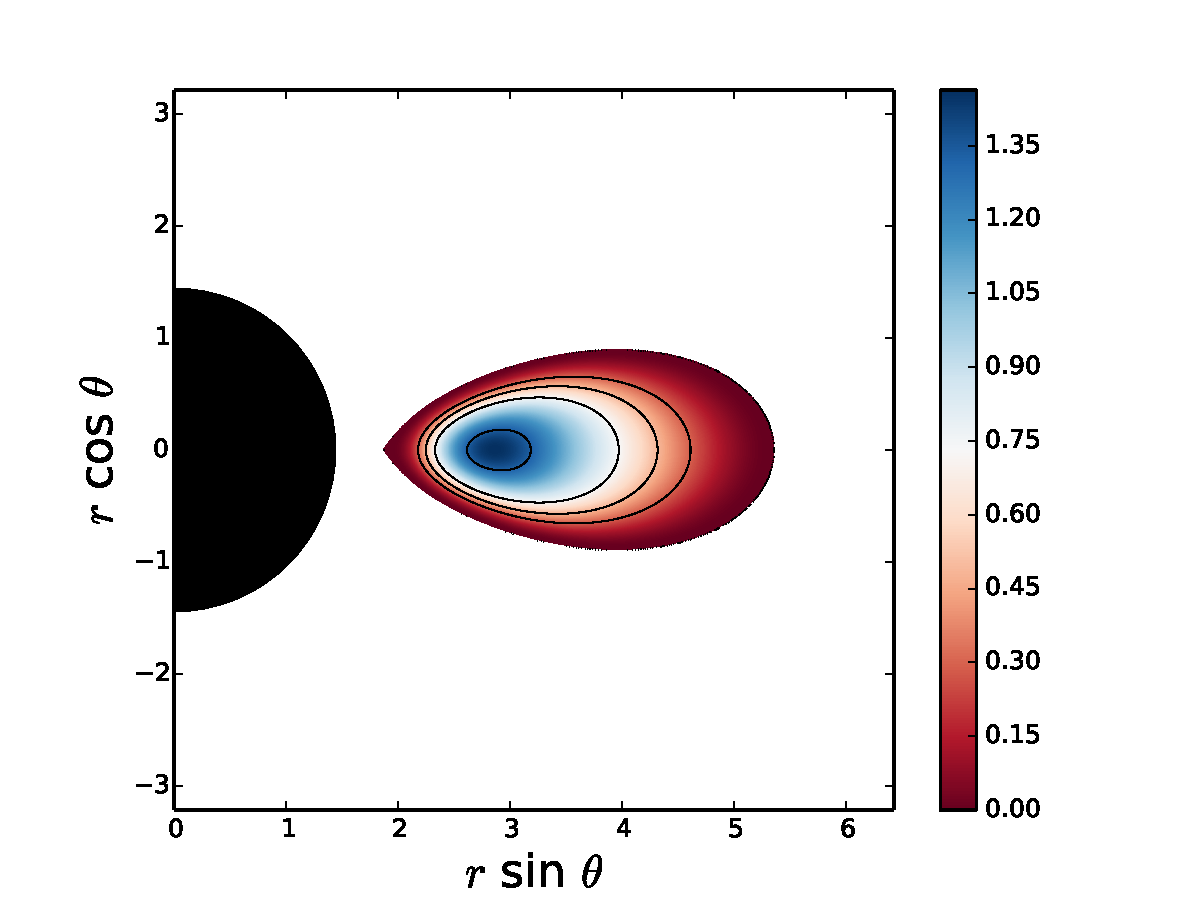
\includegraphics[scale=0.4]{images/2.pdf}
%\caption{test density plots}
%           \label{FigGam}%
% \end{figure*}

\begin{table*}
\caption{test two column table}             
\label{table:1}      
\centering          
\begin{tabular}{c c c c c c c c c c}
\hline\hline       
                      
Modelo & $\beta$ & $\gamma$ & $\beta_{\mathrm{c}}$ & $\Delta W$ & $r_{\mathrm{in}}$ & $r_{\mathrm{out}}$ & $r_{p_{\rm{max}}}$ & $r_{p_{\mathrm{mag, max}}}$ & $p_{\mathrm{max}}$\\ 
\hline                    
  B-7 & $0.5$ & $0.5$ & $10^{3}$ & $-7.29 \times 10^{-2}$ & $1.27$ & $2.50$ & $1.971$ & $2.086$ & $1.83 \times 10^{-2}$\\ 
  B-8 & $0.5$ & $0.5$ & $10^{2}$ & $-7.29 \times 10^{-2}$ & $1.27$ & $2.50$ & $1.971$ & $2.076$ & $1.82 \times 10^{-2}$\\ 
  B-9 & $0.5$ & $0.5$ & $1$ & $-7.29 \times 10^{-2}$ & $1.27$ & $2.50$ & $1.931$ & $2.047$ & $1.68 \times 10^{-2}$\\ 
  B-10 & $0.5$ & $0.5$ & $1$ & $-7.29 \times 10^{-2}$ & $1.27$ & $2.50$ & $1.761$ & $1.861$ & $1.10 \times 10^{-2}$\\ 
  B-11 & $0.5$ & $0.5$ & $10^{-1}$ & $-7.29 \times 10^{-2}$ & $1.27$ & $2.50$ & $1.641$ & $1.701$ & $2.95 \times 10^{-3}$\\ 
  B-12 & $0.5$ & $0.5$ & $10^{-2}$ & $-7.29 \times 10^{-2}$ & $1.27$ & $2.50$ & $1.621$ & $1.681$ & $3.59 \times 10^{-4}$\\ 
  B-13 & $0.5$ & $0.5$ & $10^{-3}$ & $-7.29 \times 10^{-2}$ & $1.27$ & $2.50$ & $1.611$ & $1.671$ & $3.67 \times 10^{-5}$\\ 
\hline                  
\end{tabular}
\end{table*}


%--------------------------------------------------------------------
\section{Conclusions}

%-------------------------------------- Two column figure (place early!)
%   \begin{figure*}
%   \centering
%   %%%\includegraphics{empty.eps}
%   %%%\includegraphics{empty.eps}
%   %%%\includegraphics{empty.eps}
%   \caption{Adiabatic exponent $\Gamma_1$.
%               $\Gamma_1$ is plotted as a function of
%               $\lg$ internal energy $\mathrm{[erg\,g^{-1}]}$ and $\lg$
%               density $\mathrm{[g\,cm^{-3}]}$.}
%              \label{FigGam}%
%    \end{figure*}
%


%--------------------------------------------------- One column table
%   \begin{table}
%      \caption[]{Opacity sources.}
%         \label{KapSou}
%     $$ 
%         \begin{array}{p{0.5\linewidth}l}
%            \hline
%            \noalign{\smallskip}
%            Source      &  T / {[\mathrm{K}]} \\
%            \noalign{\smallskip}
%            \hline
%            \noalign{\smallskip}
%            Yorke 1979, Yorke 1980a & \leq 1700^{\mathrm{a}}     \\
%%           Yorke 1979, Yorke 1980a & \leq 1700             \\
%            Kr\"ugel 1971           & 1700 \leq T \leq 5000 \\
%            Cox \& Stewart 1969     & 5000 \leq             \\
%            \noalign{\smallskip}
%            \hline
%         \end{array}
%     $$ 
%   \end{table}
%



\begin{acknowledgements}
      Work supported by the Spanish MINECO (grants AYA2013-40979-P and AYA2015-66899-C2-1-P) and the Generalitat Valenciana (PROMETEOII-2014-069).
\end{acknowledgements}

% WARNING
%-------------------------------------------------------------------
% Please note that we have included the references to the file aa.dem in
% order to compile it, but we ask you to:
%
% - use BibTeX with the regular commands:
%   \bibliographystyle{aa} % style aa.bst
%   \bibliography{references.bib} % your references Yourfile.bib
%
% - join the .bib files when you upload your source files
%-------------------------------------------------------------------

\bibliographystyle{bibtex/aa}
\bibliography{references}

\end{document}
